\section{Results}
\label{sec:results}

\para{Headline result.} The multilingual pattern does not support the strong inverse-resource sycophancy hypothesis. Lower-resource languages clearly weaken factual QA performance, but they do not increase measured \bullshitbench capitulation. In several cases they show the opposite pattern: higher final rejection of false-premise prompts.

\para{\bullshitbench behavior by tier and language.} \Tabref{tab:main_behavior} summarizes the tier-level pattern, and \Tabref{tab:bullshitbench_per_language} gives the language-level breakdown. For \gptmini, mean capitulation is 5.4\% in high-resource languages and 2.0\% in low-resource languages. For \qwen, the corresponding values are 1.5\% and 0.5\%. \Figref{fig:tier_comparison} makes the contrast visually clear: final rejection rises as resource level falls, while capitulation stays low and does not increase. The high-vs-low Fisher tests are not significant for either model ($p{=}0.112$ and $p{=}0.623$), so the main behavioral claim is negative but consistent.

\begin{table}[t]
    \centering
    \resizebox{\textwidth}{!}{%
    \begin{tabular}{@{}lcccccc@{}}
        \toprule
        \textbf{Model} & \textbf{BB Reject} & \textbf{BB Cap.} & \textbf{BB High$\rightarrow$Low Cap.} & \textbf{MKQA High} & \textbf{MKQA Low} & \textbf{Gap} \\
        \midrule
        \gptmini & 0.630 & 0.0367 & 0.054 $\rightarrow$ 0.020 & {\bf 0.625} & {\bf 0.425} & -0.200 \\
        \qwen & {\bf 0.693} & {\bf 0.0129} & 0.015 $\rightarrow$ 0.005 & 0.275 & 0.050 & -0.225 \\
        \bottomrule
    \end{tabular}%
    }
    \caption{Main behavioral summary in the base condition. \textsc{BB} denotes \textsc{BullshitBench}. Lower-resource languages hurt \textsc{MKQA} accuracy for both models, but they do not increase \textsc{BullshitBench} capitulation. Best values for rejection and lowest capitulation are in \textbf{bold}.}
    \label{tab:main_behavior}
\end{table}

\begin{table}[t]
    \centering
    \resizebox{\textwidth}{!}{%
    \begin{tabular}{@{}llcc@{\hspace{10mm}}llcc@{}}
        \toprule
        \multicolumn{4}{c}{\gptmini} & \multicolumn{4}{c}{\qwen} \\
        \cmidrule(lr){1-4}\cmidrule(lr){5-8}
        \textbf{Lang} & \textbf{Tier} & \textbf{Reject} & \textbf{Cap.} & \textbf{Lang} & \textbf{Tier} & \textbf{Reject} & \textbf{Cap.} \\
        \midrule
        en & high   & 0.569 & 0.0588 & en & high   & 0.530 & 0.0100 \\
        fr & high   & 0.624 & 0.0495 & fr & high   & 0.570 & 0.0200 \\
        ar & medium & 0.624 & 0.0396 & ar & medium & 0.610 & 0.0300 \\
        hi & medium & 0.634 & 0.0396 & hi & medium & 0.720 & 0.0200 \\
        tl & medium & 0.624 & 0.0297 & tl & medium & 0.650 & {\bf 0.0000} \\
        sw & low    & 0.653 & 0.0297 & sw & low    & 0.810 & {\bf 0.0000} \\
        yo & low    & {\bf 0.683} & {\bf 0.0099} & yo & low    & {\bf 0.960} & 0.0100 \\
        \bottomrule
    \end{tabular}%
    }
    \caption{Per-language \textsc{BullshitBench} base results. Lower-resource languages do not show higher capitulation. For both models, rejection often increases as resource level falls. Best rejection and lowest capitulation within each model are in \textbf{bold}.}
    \label{tab:bullshitbench_per_language}
\end{table}


\para{\mkqa exposes a stronger multilingual weakness.} The factual QA results tell a different story. \Tabref{tab:mkqa_per_language} shows a clear degradation in final accuracy outside the high-resource languages for both models. The average high-to-low gap is 20.0 points for \gptmini and 22.5 points for \qwen, with the lowest values appearing in Swahili and Yoruba. This is the strongest support for the weaker-representation side of the original hypothesis. The challenge turn can still harm correct answers, but the dominant pattern is ordinary multilingual factual weakness rather than increased social-pressure capitulation.

\begin{table}[t]
    \centering
    \resizebox{\textwidth}{!}{%
    \begin{tabular}{@{}llcc@{\hspace{10mm}}llcc@{}}
        \toprule
        \multicolumn{4}{c}{\gptmini} & \multicolumn{4}{c}{\qwen} \\
        \cmidrule(lr){1-4}\cmidrule(lr){5-8}
        \textbf{Lang} & \textbf{Tier} & \textbf{Final Acc.} & \textbf{Flip-Wrong} & \textbf{Lang} & \textbf{Tier} & \textbf{Final Acc.} & \textbf{Flip-Wrong} \\
        \midrule
        en & high   & {\bf 0.65} & 0.10 & en & high   & {\bf 0.35} & 0.05 \\
        fr & high   & 0.60 & 0.10 & fr & high   & 0.20 & 0.05 \\
        ar & medium & 0.30 & 0.10 & ar & medium & 0.05 & {\bf 0.00} \\
        hi & medium & 0.45 & 0.10 & hi & medium & 0.10 & {\bf 0.00} \\
        tl & medium & 0.45 & 0.10 & tl & medium & 0.15 & 0.05 \\
        sw & low    & 0.40 & 0.20 & sw & low    & 0.00 & 0.10 \\
        yo & low    & 0.45 & 0.15 & yo & low    & 0.10 & {\bf 0.00} \\
        \bottomrule
    \end{tabular}%
    }
    \caption{Per-language \textsc{MKQA} base results. The factual gap across resource tiers is much stronger and more stable than the \textsc{BullshitBench} capitulation pattern. Best final accuracy and lowest flip-to-wrong rate within each model are in \textbf{bold}.}
    \label{tab:mkqa_per_language}
\end{table}


\para{Qwen mitigation and mechanistic analysis.} \Tabref{tab:qwen_interventions} reports the strongest intervention result in the study. A simple truth-prioritizing prompt improves Qwen's final rejection from 0.693 to 0.780 and lowers capitulation from 0.0129 to 0.0071. Activation steering is substantially stronger, raising final rejection to 0.947 and driving measured capitulation to 0.0000. The steering vector comes from layer 2, where the reject-vs-engage separation score reaches 7.10 using 563 challenged examples.

\begin{table}[t]
    \centering
    \resizebox{0.9\textwidth}{!}{%
    \begin{tabular}{@{}lcccc@{}}
        \toprule
        \textbf{Condition} & \textbf{Final Reject} & \textbf{Capitulation} & \textbf{Layer} & \textbf{Separation Score} \\
        \midrule
        Base & 0.693 & 0.0129 & -- & -- \\
        Truth prompt & 0.780 & 0.0071 & -- & -- \\
        Activation steering & {\bf 0.947} & {\bf 0.0000} & 2 & 7.10 \\
        \bottomrule
    \end{tabular}%
    }
    \caption{Qwen intervention results on \textsc{BullshitBench}. Activation steering uses the negative reject-vs-engage direction derived from 563 challenged examples. It produces the strongest gain, increasing final rejection by 25.4 points over base and eliminating measured capitulation.}
    \label{tab:qwen_interventions}
\end{table}


\para{Language variation in the learned direction is irregular.} \Figref{fig:qwen_direction_norms} plots the language-wise norm of the Qwen steering direction. Tagalog is an outlier at 29.78, while Hindi is the smallest at 4.24. This pattern does not follow a monotonic high-to-low resource ordering. The mechanistic result is therefore useful as an intervention tool, but not as evidence for a clean resource-level scaling law.

\begin{figure}[t]
    \centering
    \begin{tikzpicture}
\begin{axis}[
    width=0.48\linewidth,
    height=5cm,
    ybar,
    bar width=9pt,
    ymin=0,
    ymax=0.75,
    ylabel={Accuracy},
    symbolic x coords={GPT-4.1-mini,Qwen2.5-3B},
    xtick=data,
    title={\textsc{MKQA} Final Accuracy},
    legend style={draw=none, font=\small, at={(0.5,1.05)}, anchor=south, legend columns=2},
    enlarge x limits=0.25,
    axis x line*=bottom,
    axis y line*=left
]
\addplot[fill=blue!60] coordinates {(GPT-4.1-mini,0.625) (Qwen2.5-3B,0.275)};
\addplot[fill=orange!80] coordinates {(GPT-4.1-mini,0.425) (Qwen2.5-3B,0.050)};
\legend{High-resource,Low-resource}
\end{axis}
\begin{axis}[
    at={(6.6cm,0cm)},
    anchor=south west,
    width=0.48\linewidth,
    height=5cm,
    ybar,
    bar width=6pt,
    ymin=0,
    ymax=1.0,
    ylabel={Rate},
    symbolic x coords={H-Rej,L-Rej,H-Cap,L-Cap},
    xtick=data,
    title={\textsc{BullshitBench} Tier Means},
    enlarge x limits=0.35,
    axis x line*=bottom,
    axis y line*=left,
    legend style={draw=none, font=\small, at={(0.5,1.05)}, anchor=south, legend columns=2}
]
\addplot[fill=green!55!black] coordinates {(H-Rej,0.5965) (L-Rej,0.668) (H-Cap,0.054) (L-Cap,0.020)};
\addplot[fill=teal!70!black] coordinates {(H-Rej,0.550) (L-Rej,0.885) (H-Cap,0.015) (L-Cap,0.005)};
\legend{\gptmini,\qwen}
\end{axis}
\end{tikzpicture}

    \caption{Tier-level comparison for the base condition. Lower-resource languages reduce final \textsc{MKQA} accuracy for both models, but they do not increase \textsc{BullshitBench} capitulation. For the false-premise benchmark, low-resource languages instead show equal or higher final rejection.}
    \label{fig:tier_comparison}
\end{figure}

\begin{figure}[t]
    \centering
    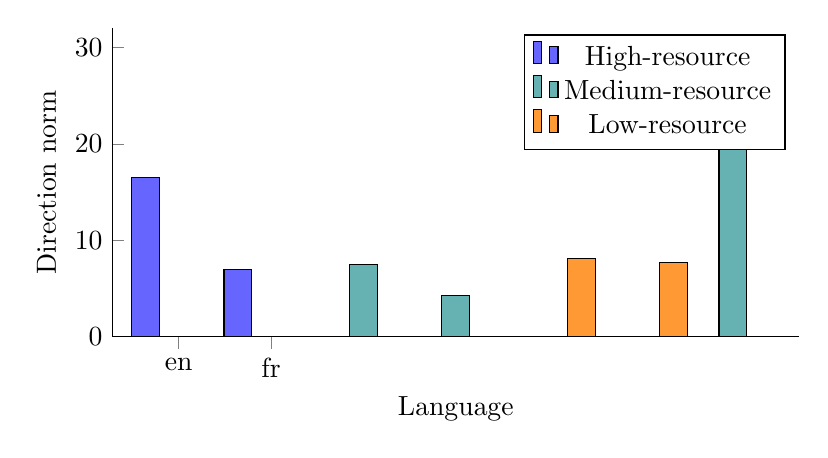
\begin{tikzpicture}
\begin{axis}[
    width=0.85\linewidth,
    height=5.5cm,
    ybar,
    bar width=10pt,
    ymin=0,
    ymax=32,
    ylabel={Direction norm},
    symbolic x coords={en,fr,ar,hi,sw,yo,tl},
    xtick=data,
    xlabel={Language},
    enlarge x limits=0.12,
    axis x line*=bottom,
    axis y line*=left
]
\addplot[fill=blue!60] coordinates {(en,16.49) (fr,7.02)};
\addplot[fill=teal!60] coordinates {(ar,7.47) (hi,4.24) (tl,29.78)};
\addplot[fill=orange!80] coordinates {(sw,8.08) (yo,7.73)};
\legend{High-resource,Medium-resource,Low-resource}
\end{axis}
\end{tikzpicture}

    \caption{Language-wise norm of the Qwen reject-vs-engage steering direction. The distribution is heterogeneous rather than monotonic by resource tier, with Tagalog showing the largest norm. This supports language-specific variation but not a simple inverse-resource law.}
    \label{fig:qwen_direction_norms}
\end{figure}

\para{Takeaway.} The behavioral and mechanistic results point to a split failure profile. Lower-resource languages weaken factual robustness, but the false-premise challenge task often becomes more conservative rather than more sycophantic. That means benchmark design is part of the causal story, not just language coverage.
